\documentclass{article}

\usepackage{amsmath}
\usepackage{graphicx}

\graphicspath{ {./images/} }

\title{Physics 642 - Stat Mech 2: Phase Transitions and Critical Phenomena - Final Project Report}
\author{Cary Rock}
\date{\today}

\begin{document}
    \maketitle

    \section{A - \textit{L = 16}}
        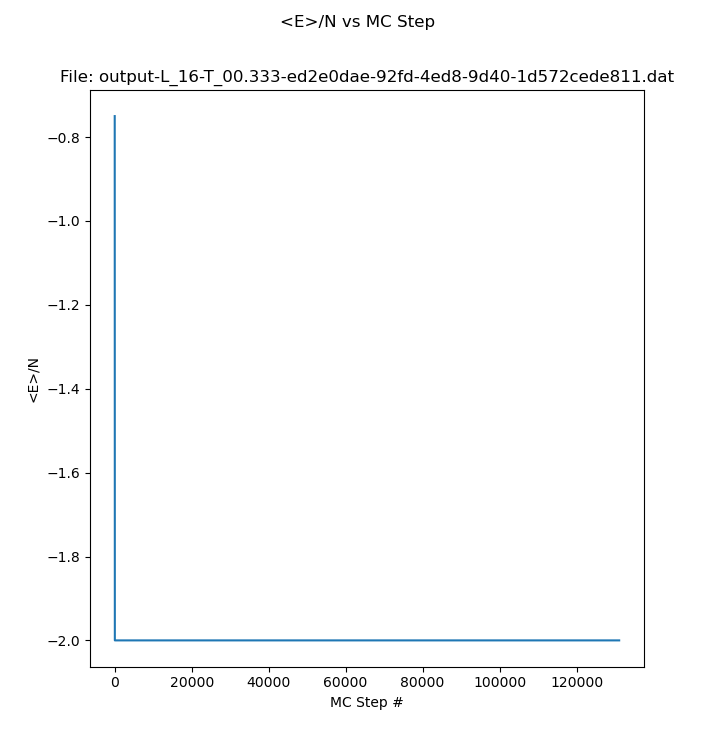
\includegraphics[width=0.5\textwidth]{A/A-E-0_333}
        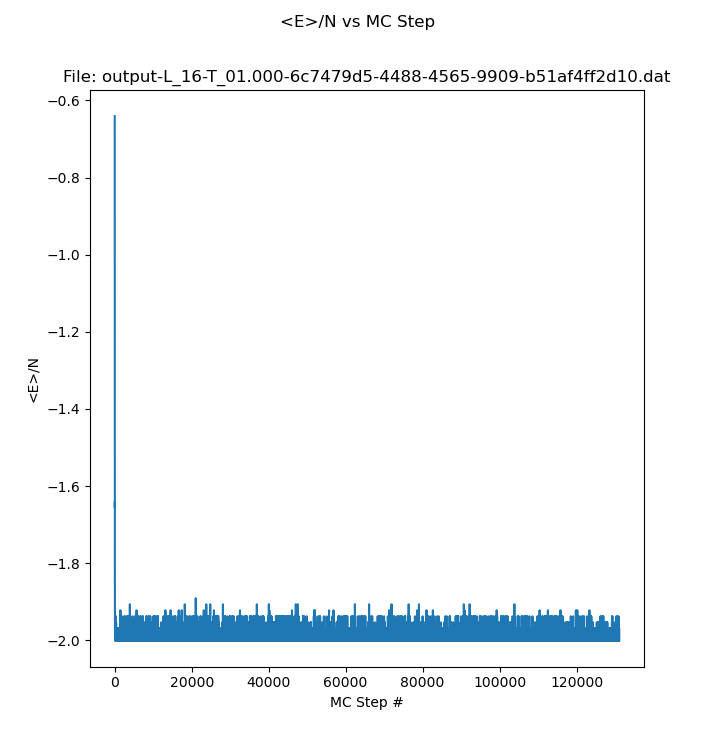
\includegraphics[width=0.5\textwidth]{A/A-E-1_000}
        
        As can be seen by the two graphs, the warm up period is rather short - for any appreciable number of steps, the system has definitely reached equilibriation.
        
    \section{B - $\frac{\langle E \rangle}{N} $ and $ \frac{\langle M \rangle}{N} $}
    	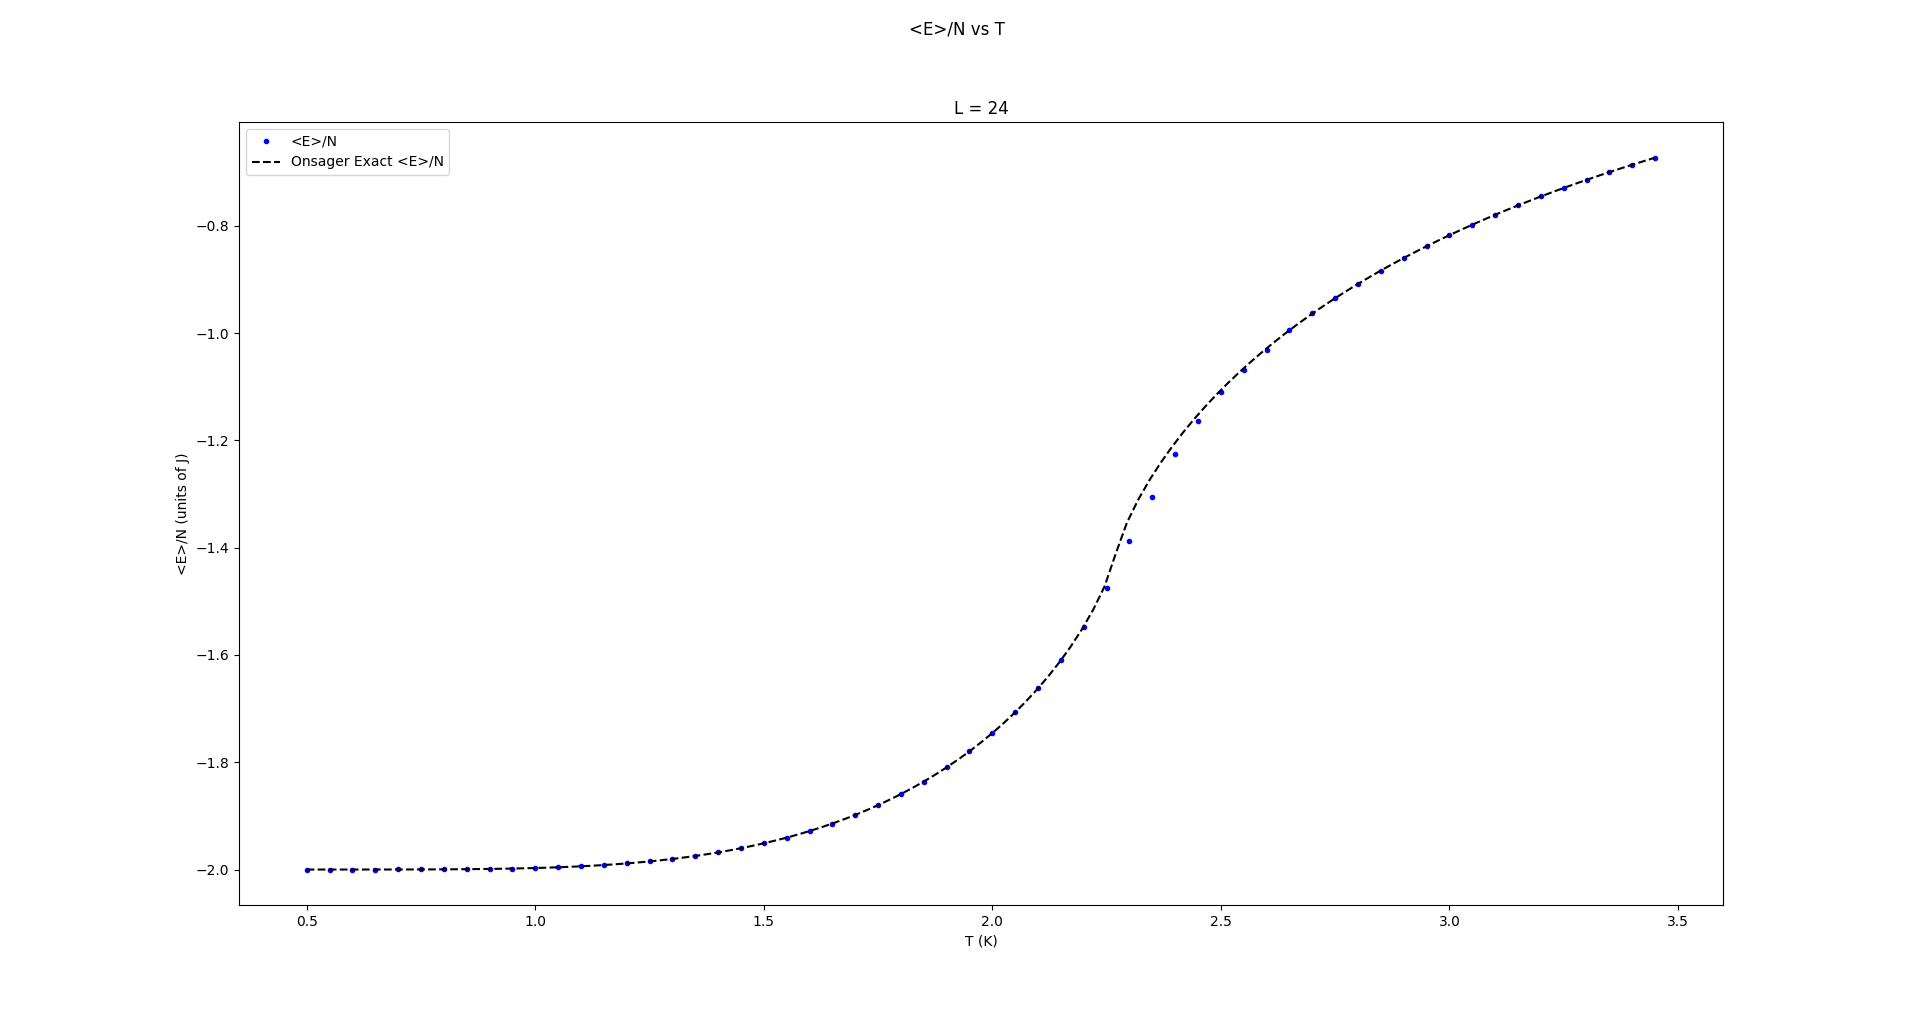
\includegraphics[width=\textwidth]{B/B-24-EoNvT} 
    	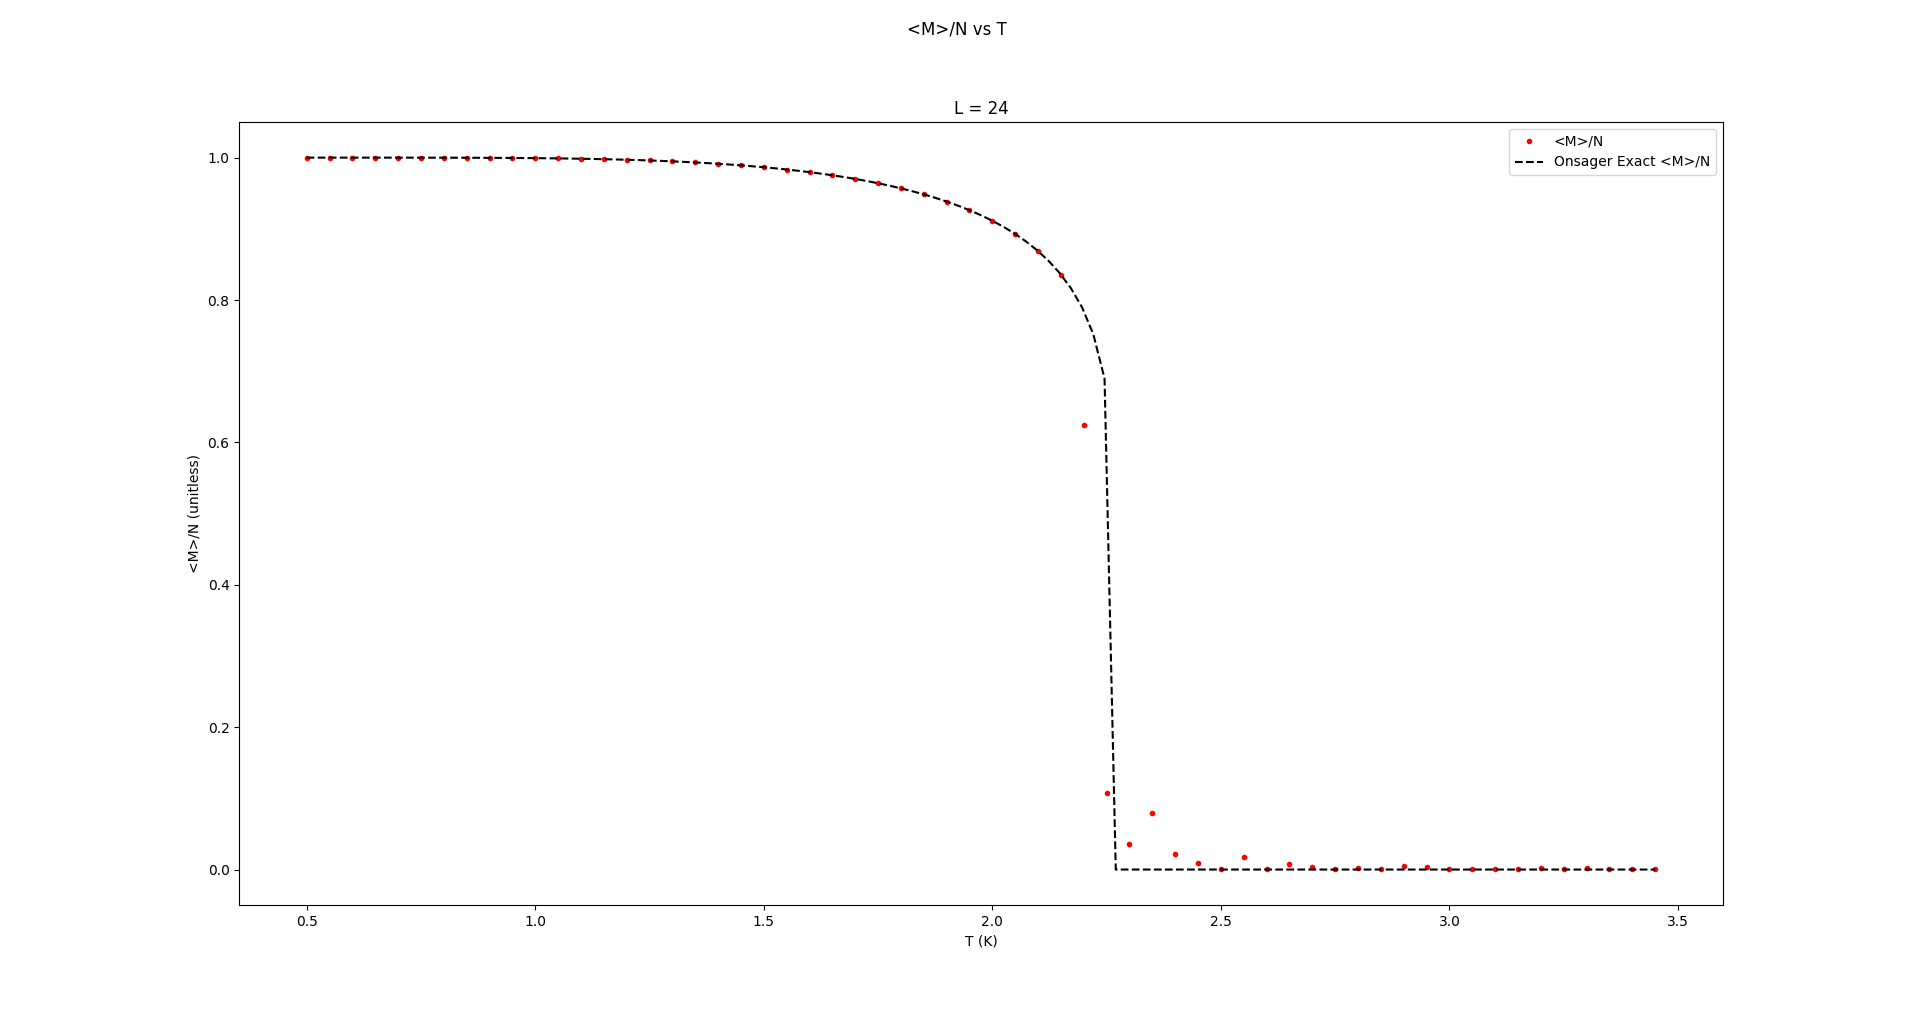
\includegraphics[width=\textwidth]{B/B-24-MoNvT}
    	
    	Yes. Included in this report above are the graphs for $\frac{\langle E \rangle}{N} $ and $ \frac{\langle M \rangle}{N} $ at side length $ L = 24 $ sites, though \cite{crock2} contains the graphs for $ L = 12\text{, }16\text{, and }20$. As can be seen from the graphs themselves, the simulation seems to follow the theoretical values predicted by Onsager for both $ \lim T \rightarrow \infty $ and $ \lim T \rightarrow 0 $. The most notable section of disagreement, such as it is, is around the critical temperature. Around this region (specifically, around the temperature $ T_C = \frac{2}{\ln(1+\sqrt{2})} \approx 2.269... K $), the magnetization jumps sharply due to the effects of the diverging correlation length making themselves known. The simulation employs the Mean Field approximation, so it is not as `sharp' as the analytic in terms of its acquiring of a non-zero magnetic moment.

    \section{C - Specific Heat, $ C_V $}
		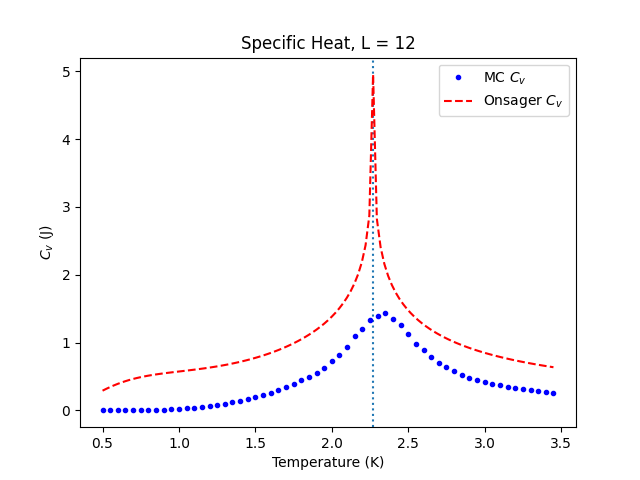
\includegraphics[width=\textwidth]{C/C_12}
		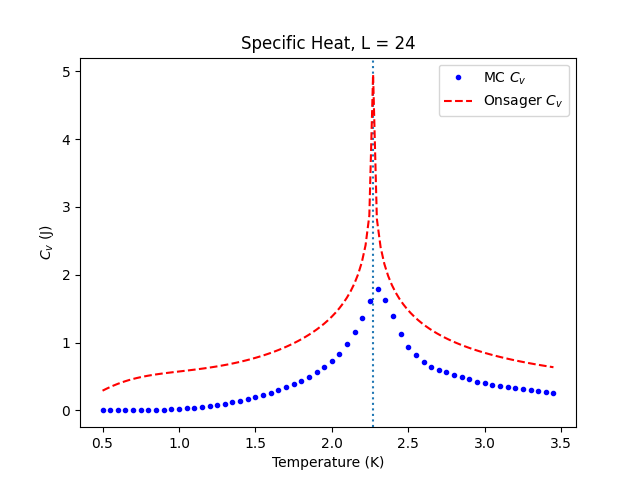
\includegraphics[width=\textwidth]{C/C_24}
		In these graphs, the blue dots represent the simulation's data, while the red line is Onsager's exact solution. For side lengths $ L = 16,\ 20,\text{ and } 24 $, the closed temperature that the data could claim as being $ T_C $ was $ 2.3 K $, which is a $ 1.36 \% $ difference from the actual. The $ L = 12 $ simulation claimed that $ T_C = 2.35 $ (a \%-difference of ~$3.56 \%$ from the actual value).
		
		A notable feature that stands out in these two included graphs (and in the ones included in \cite{crock2}) is that, while they are qualitatively similar to the analytic solutions, they miss some of the finer details (such as the changing curves for $ T < T_C $ in the exact). The reason for this inaccuracy on the part of the simulation is due again to it utilizing the mean field approximation.
		
    \section{D - Susceptibility, $ \chi_M $}
    	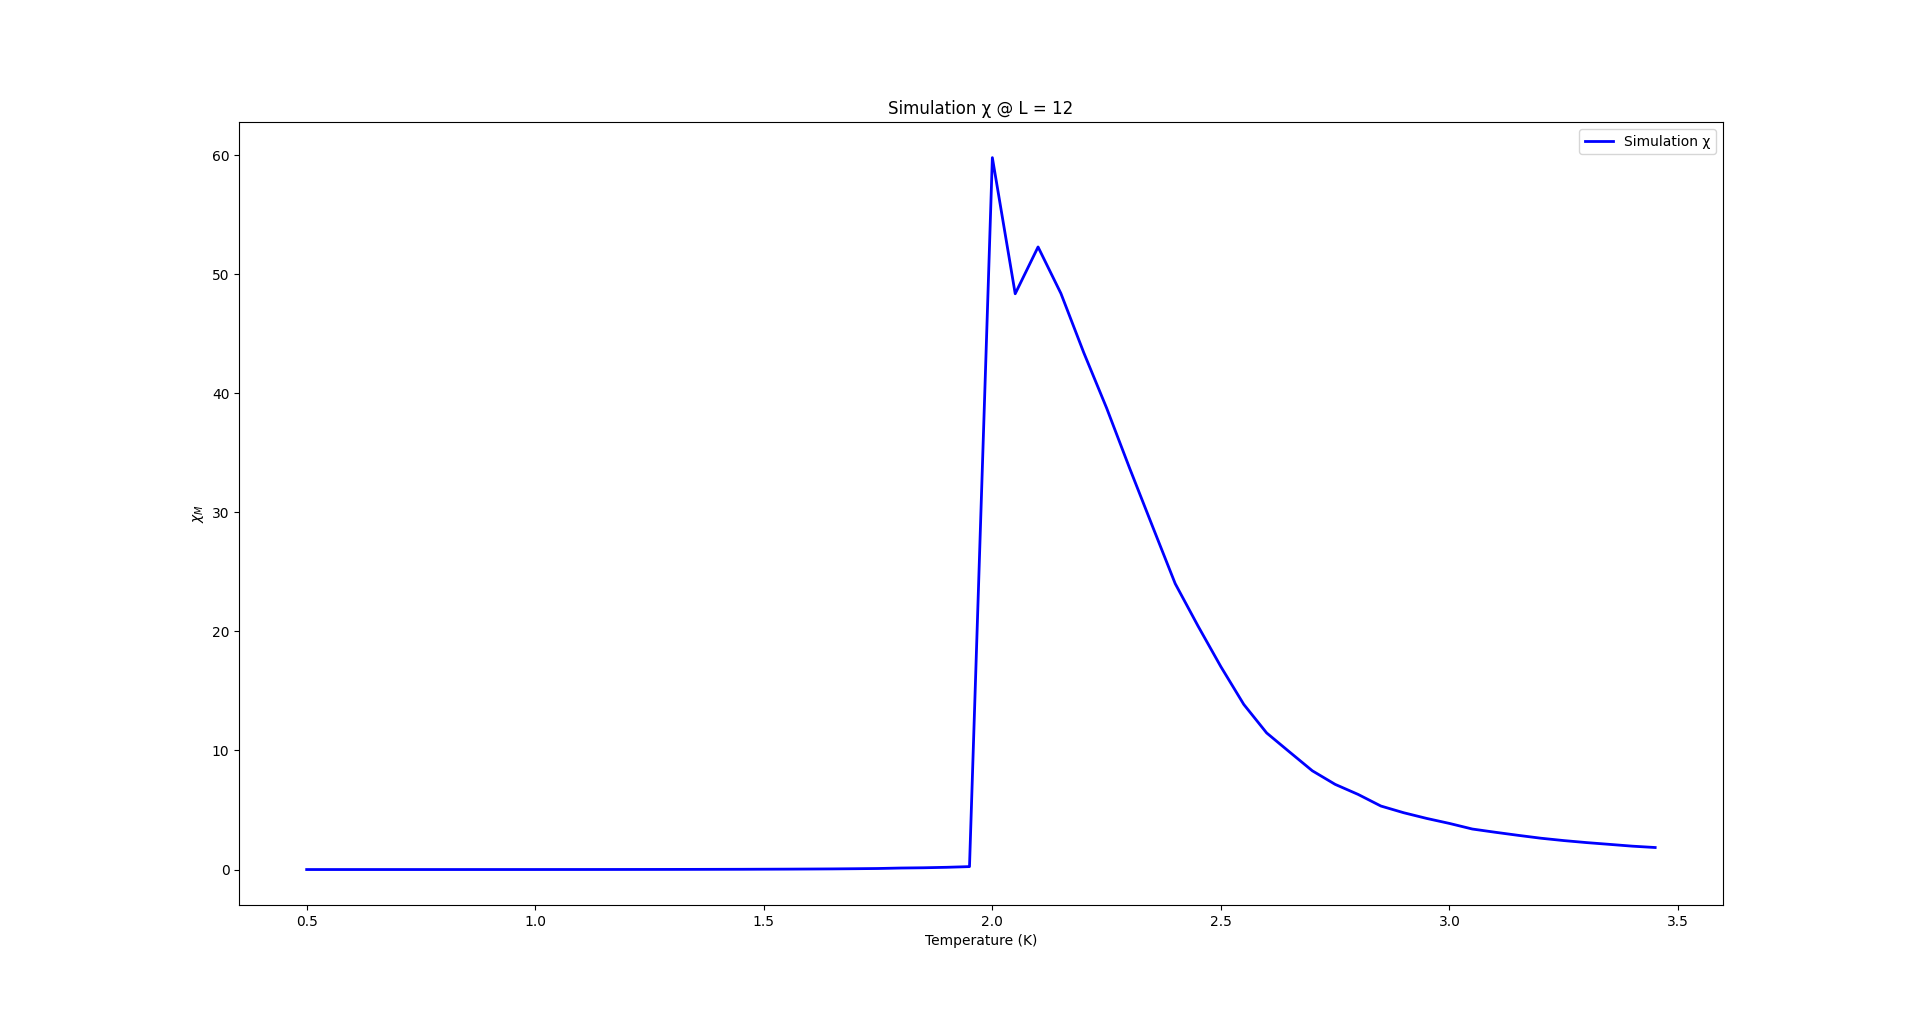
\includegraphics[width=\textwidth]{D/D-L_12}
    	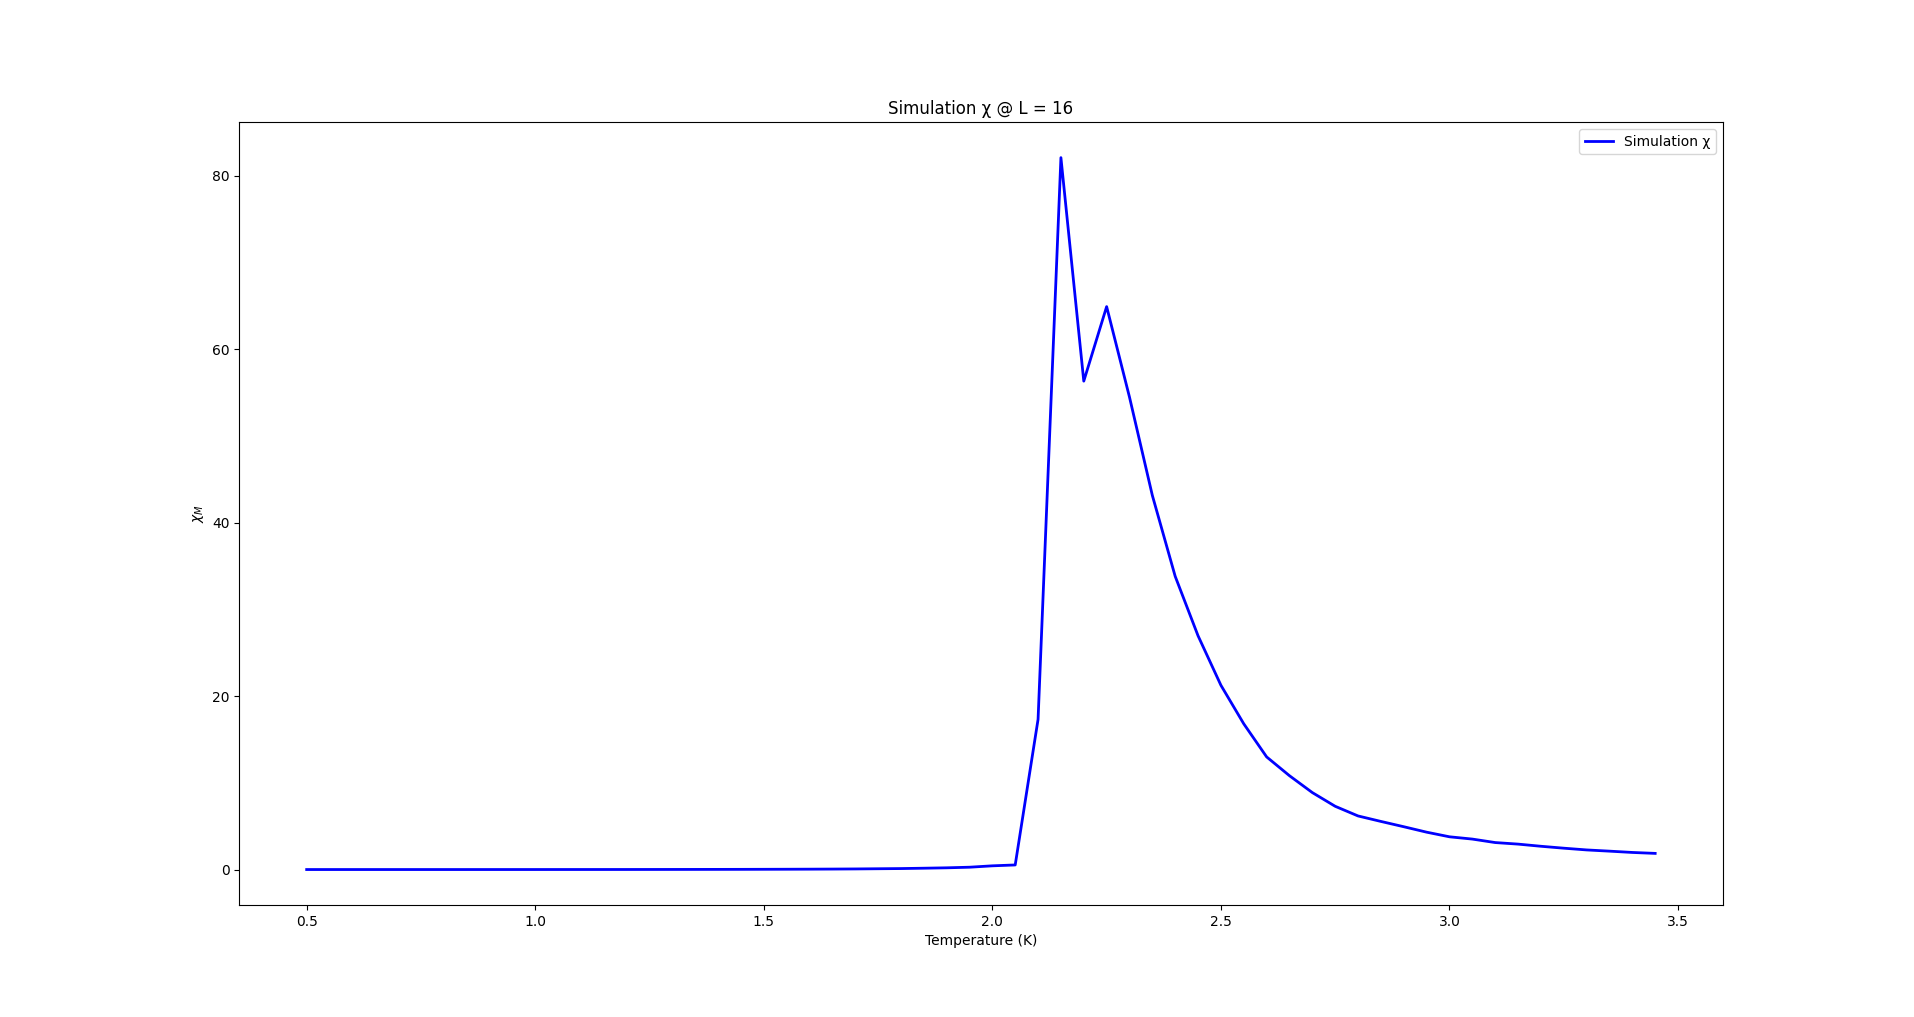
\includegraphics[width=\textwidth]{D/D-L_16}
    	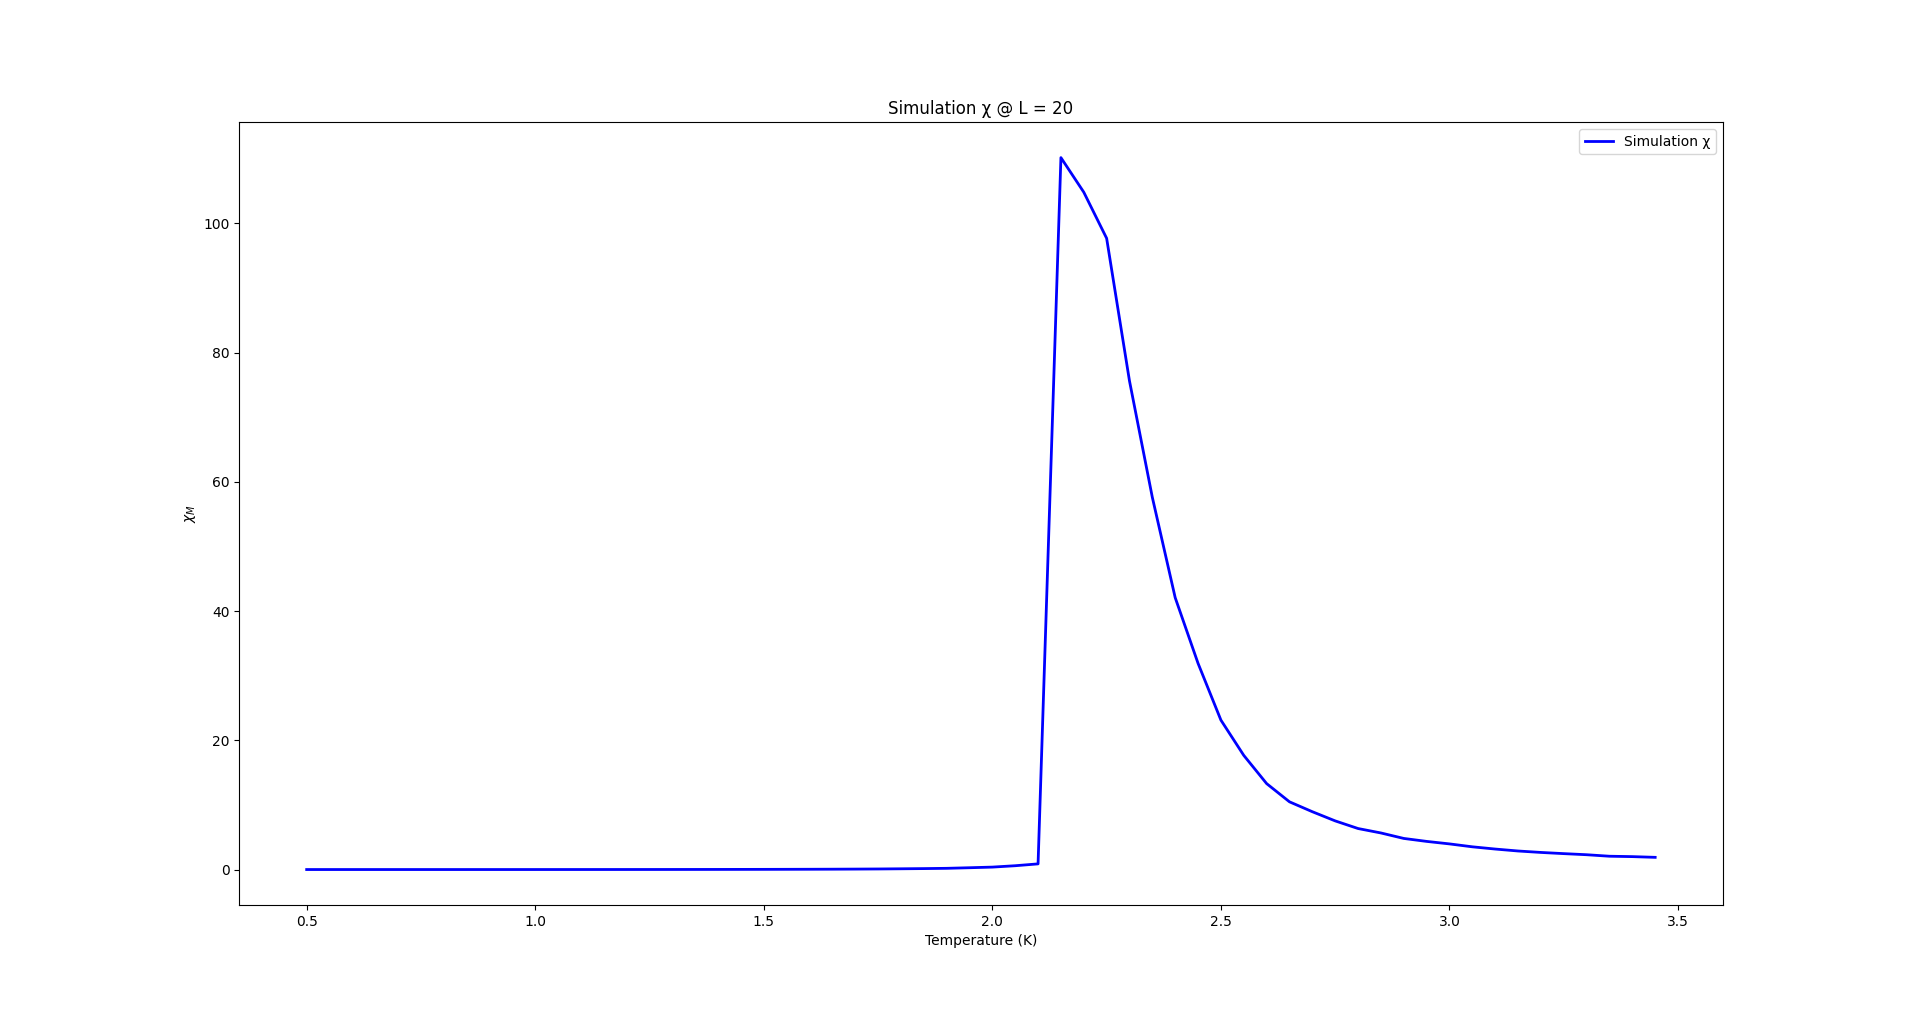
\includegraphics[width=\textwidth]{D/D-L_20}
    	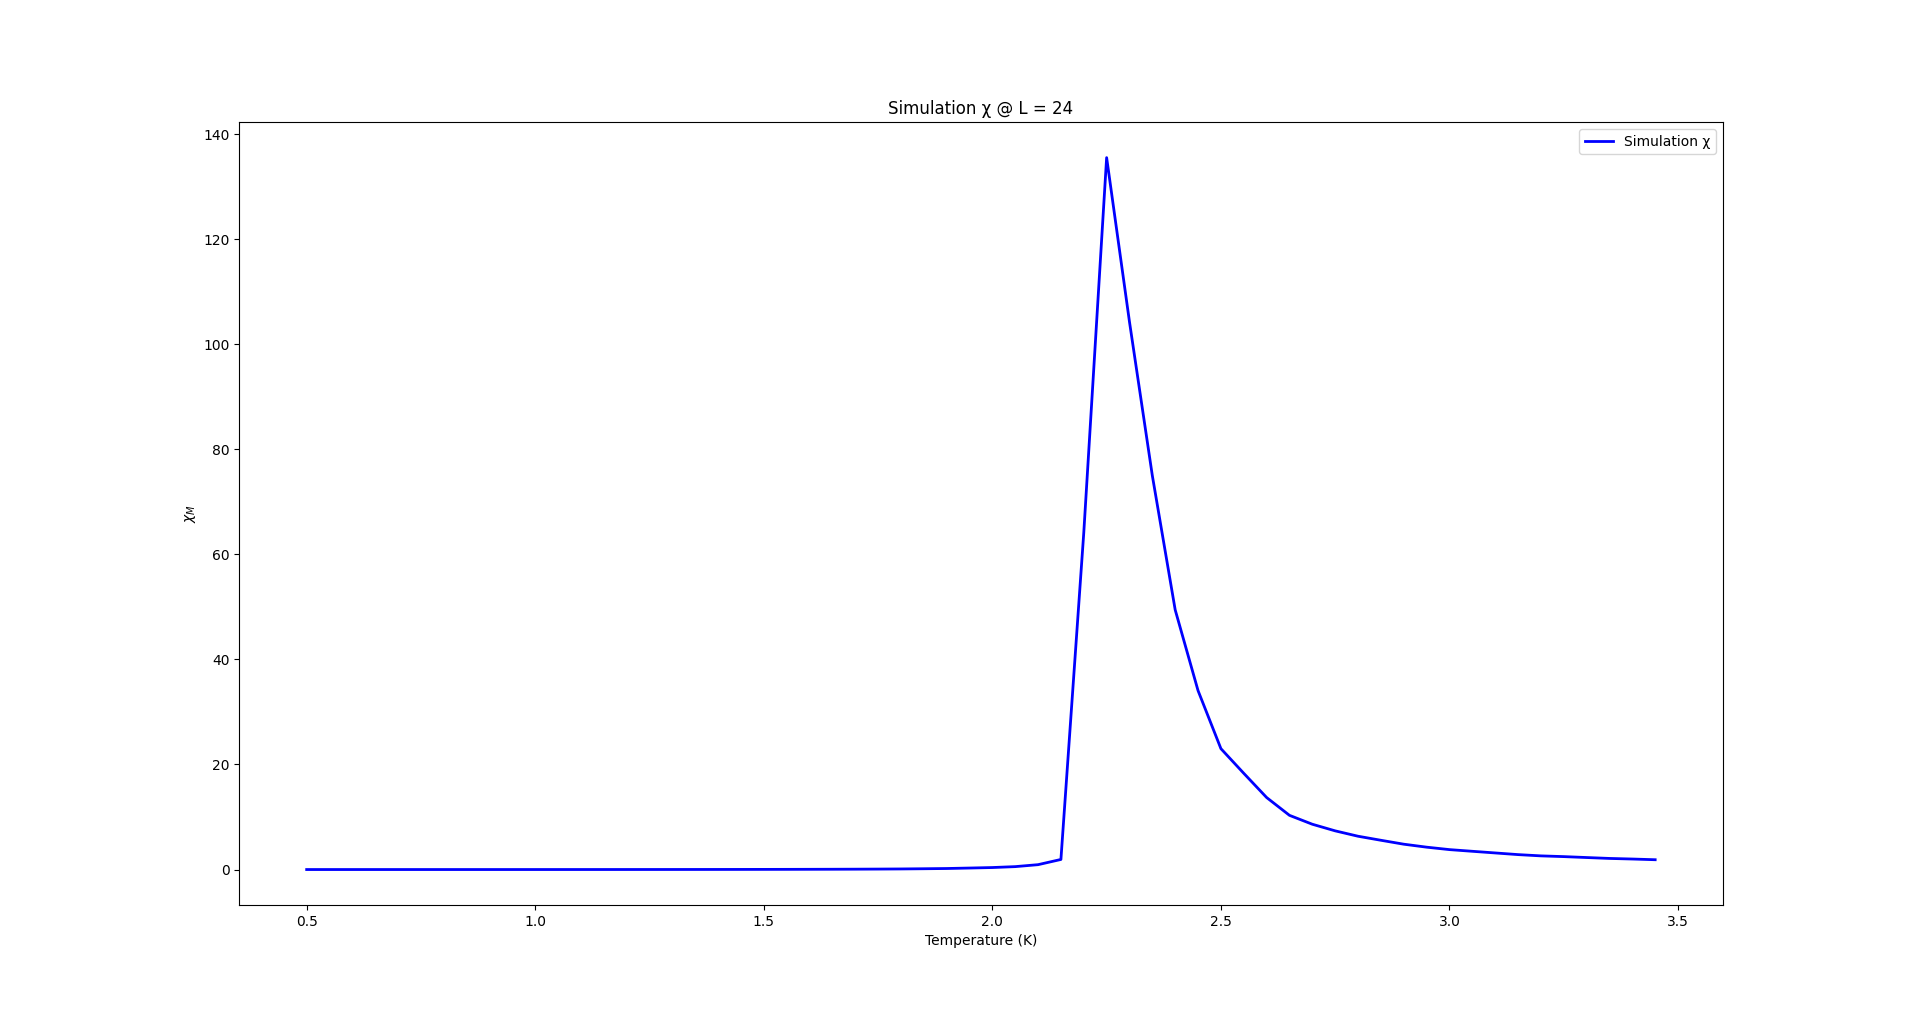
\includegraphics[width=\textwidth]{D/D-L_24}
    	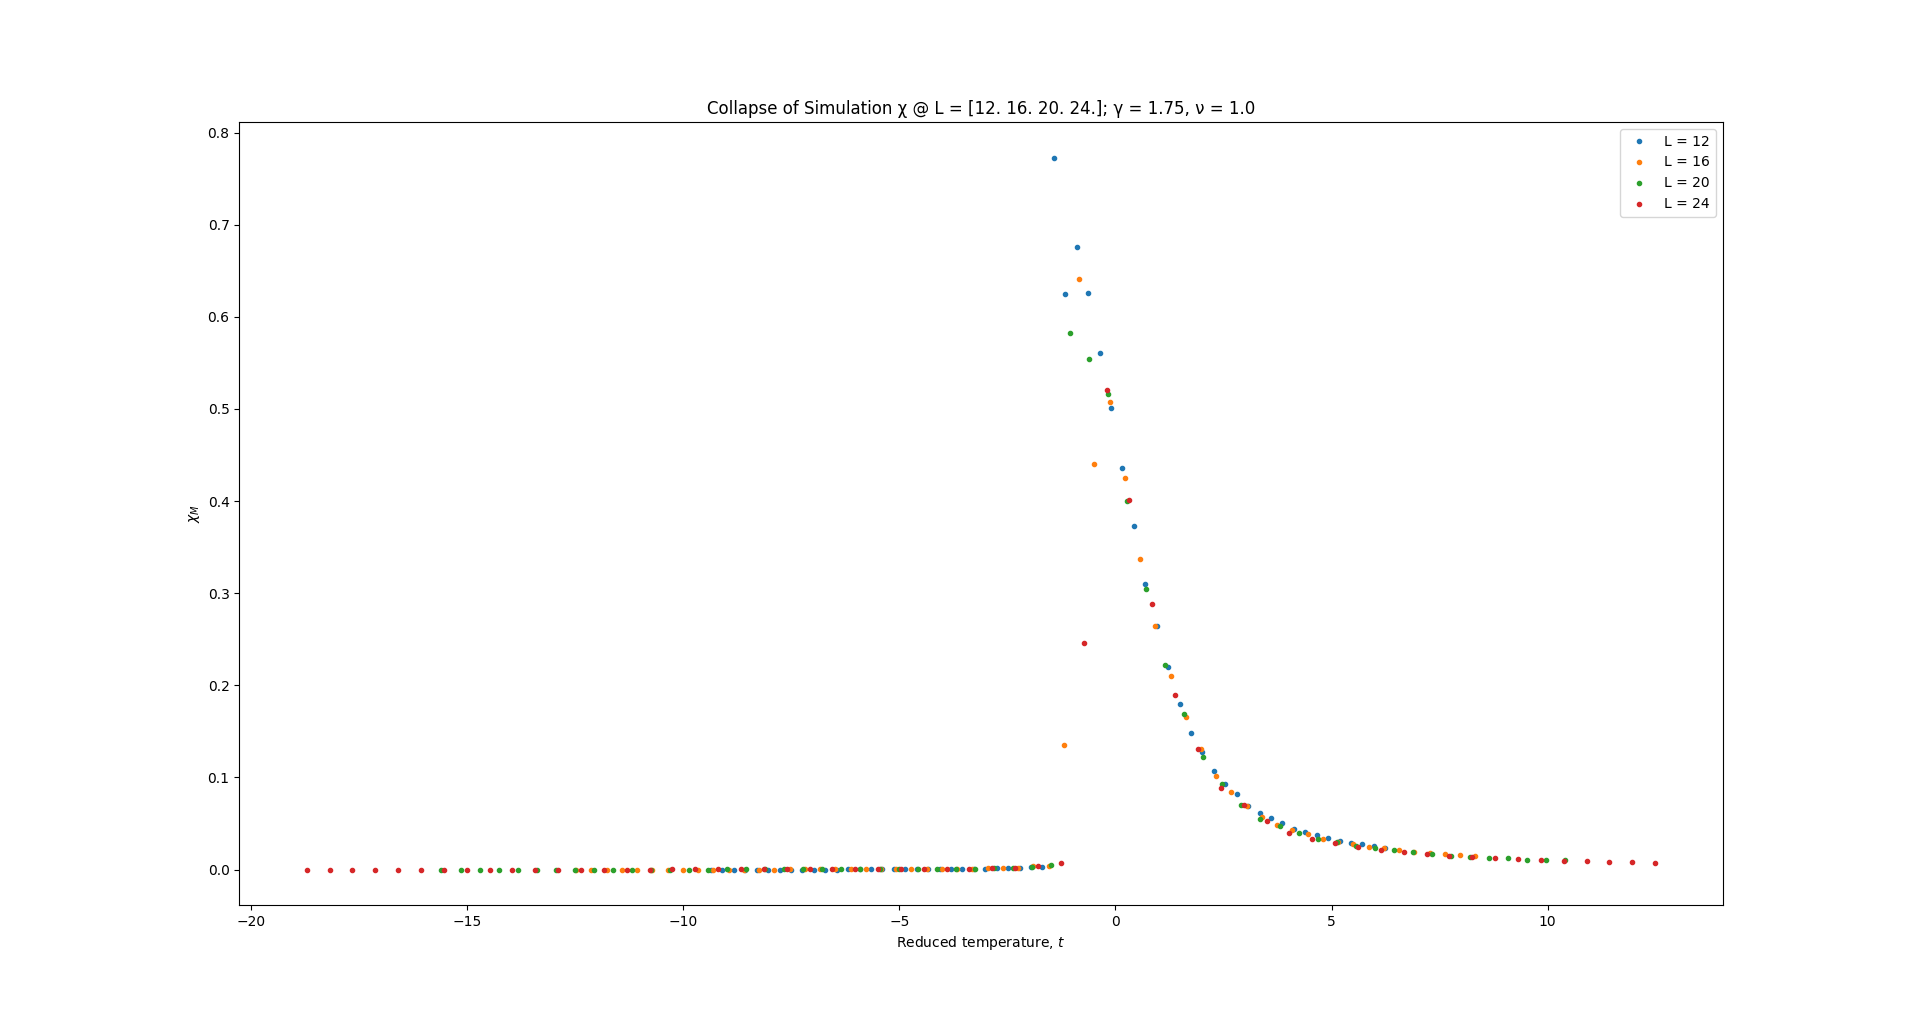
\includegraphics[width=\textwidth]{D/D-Data_collapse}
		
		Values of $\gamma \approx 1.8 \text{ and } \nu \approx 1 $ were obtained by the visual inspection of ``fitness'' by inserting trial values. A perhaps more honest approximation for $\gamma$ would be that it is, at least according to these graphs, $ 1.5 < \gamma < 2.0 $ while $ \nu $ was assumed to be $ \nu = 1 $ in a fruitless bid to compute some value algebraically. The exact values are, to two decimal places, $ \gamma = 1.75 \text{ and } \nu = 1.00 $. As can be seen from both the individual plots as well as the ``data-collapsed'' plot, larger system sizes (and more temperatures) would be required to approach the known values from this simulation.
		
		And to specifically mention sources of error as to why the graphs do not both line up nicely as well as why they are so rough individually, the predominant source of error would be due to (a lack of) statistics: there are too few simulations over an insufficient density of temperatures at too few system sizes). Increasing the number of temperature simulations run as well as increasing the system size would provide a significant increase in both accuracy of answer and precision of result. Further, a second source of error would be that each ``run'' was taken only once - a given pair of temperature and system size was performed only once. Even simply running each configuration multiple times and (at the least) averaging over the results before performing the analysis would also increase precision. 
		
	\begin{thebibliography}{100}
		\bibitem{crock2} https://github.com/CaryRock/Phys642\_Final\_Project
	\end{thebibliography}
\end{document}

